\subsection{Gerarchie}

Le classi di entità possono essere organizzate in una gerarchia di
\emph{specializzazione}. Una classe della gerarchia minore viene chiamata
\textbf{\textcolor{purple}{sottoclasse}}, mentre le altre si chiamano
\textbf{\textcolor{purple}{superclassi}}. Gli elementi di una sottoclasse
sono un sottoinsieme degli elementi della superclasse.

\subsubsection{Tipi Oggetto}

Fra i \emph{tipi oggetto} viene definita una relazione di sottotipo, che comprende le seguenti proprietà:
\begin{itemize}
    \item È una relazione \textcolor{purple}{asimmetrica}, \textcolor{purple}{riflessiva} e
        \textcolor{purple}{transitiva}.
    \item Inoltre, se un tipo $T$ è \emph{\textcolor{purple}{sottotipo}} di $T'$, allora
        tutti gli elementi di $T$ possono essere usati in tutti i contesti in cui appaiono elementi
        di tipo $T'$. Questa proprietà è chiamata \textcolor{purple}{sostitutività} ed è data dal fatto
        che gli elementi di $T$ hanno tutte le proprietà degli elementi di $T'$, e per ogni proprietà di $T'$,
        il suo tipo in $T$ è un sottotipo di quello che ha in $T'$. 
\end{itemize}

\paragraph{\textcolor{purple}{Ereditarietà}} L'\emph{ereditarietà} è una proprietà delle gerarchie
che permette di definire un \emph{tipo oggetto} a partire da un altro. In quanto, nel nostro contesto,
a partire da un tipo, si vuole solo definire un sottotipo, si parla di \emph{ereditarietà stretta}, che permette solo:
\begin{itemize}
    \item L'aggiunta di altri \emph{attributi}.
    \item La ridefinizione di attributi del \emph{supertipo}, però solo specializzando ulteriormente il tipo dell'attributo.
\end{itemize}

\subsubsection{Classi}

Fra le \emph{classi}, invece, viene definita una relazione di sottoclasse, con le seguenti proprietà:
\begin{itemize}
    \item Sempre \textcolor{purple}{asimmetrica}, \textcolor{purple}{riflessiva} e
        \textcolor{purple}{transitiva}, come per i \emph{tipi oggetto}.
    \item Se una classe $C$ è \emph{\textcolor{purple}{sottoclasse}} di $C'$, allora il tipo degli elementi di
        $C$ è sottotipo del tipo degli elementi di $C'$ (\textbf{\textcolor{purple}{vincolo intensionale}}).
    \item Se $C$ è \emph{\textcolor{purple}{sottoclasse}} di $C'$, allora gli elementi di $C$ sono un sottoinsieme
        degli elementi di $C'$ (\textbf{\textcolor{purple}{vincolo estensionale}}).
\end{itemize}

\paragraph{\textcolor{purple}{Vincoli}} Possiamo distinguere due tipi di vincoli su insiemi di sottoclassi:
\begin{itemize}
    \item \textcolor{purple}{Disgiunzione}: ogni coppia di sottoclassi nell'insieme è \emph{disgiunta}, quindi è priva di elementi comuni.
    \item \textcolor{purple}{Copertura}: l'unione degli elementi delle sottoclassi coincide con l'insieme degli elementi della \emph{superclasse}.
\end{itemize}

Se possiedono entrambi i vincoli, allora l'insieme delle \emph{sottoclassi} forma una \textcolor{purple}{partizione} della \emph{superclasse}. Altrimenti se nessuno
dei due vincoli è rispettato, si dice che le sottoclassi sono \textcolor{purple}{scorrelate}.

\begin{figure}[h]
    \centering
    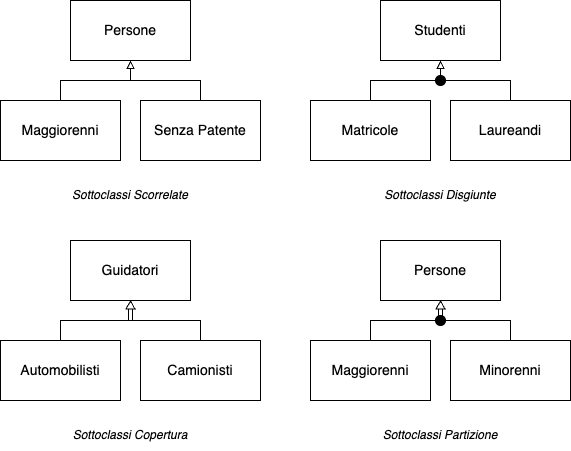
\includegraphics[scale=0.6]{img/gerarchie.png}
\end{figure}

\subsubsection{Ereditarietà Multipla}

Un tipo può anche essere definito per \emph{ereditarietà} anche a partire da più di un
\emph{supertipo}. Questo però può creare alcuni problemi quando lo stesso \emph{attributo} viene ereditato
da più di un supertipo, ma i tipi degli attributi fra loro sono diversi.